\chapter{High-Level Design Principles}

Welcome to the opinionated part of this text. Like many opinions, they're held for particular reasons, and made by a human rather than divine intervention. The best you can hope is that I've been divinely inspired, so ask yourself constantly, "does this make sense?"

A lot of this first chapter in design will be thinking about the design process itself, rather than the actual objects being designed. This may sound like it falls under the pervue of philosophy (which may drive you to boredom or an existential crisis), and it does! But it is practical philosophy.

\section{Designing a Project}

I'll say project, and not team because some projects are done by individuals, and projects are bigger than teams. There's a lot of adages about project management. This is not a project management book and doesn't set out to be, but the fact of the matter is that project management influences technical design, to the chagrin of many engineers. Management is wed to engineering, and the divorce is always an ugly one. May as well be good bedfellows, and make a happy marriage.

What you can do in a project should always be considered. There are a number of mantras which dwell on this:

\begin{asparaitem}
	\item ``Good, fast, or cheap: choose two." (The delusional will realize ``none" is also an option.)
	\item ``A robot with 1 mechanism at 100\% is better than 10 working at 10\%"
	\item ``The first 80\% of the task can be accomplished with 20\% of the work."
\end{asparaitem}

\section{Designing Metrics}

A lot of my thoughts on high level design and metrics are grafted from the world of software. Gary Berndhart's \href{https://www.destroyallsoftware.com/talks/boundaries}{\color{red}\underline{Boundaries}} is a particularly good example of this because it highlights what so many engineers do wrong in their testing and design. The essential problem is that they get locked into a particular set of units which must exist, and so metrics are formed based around these units rather than end results.

%There are a number of fallacies people make about metrics:
%- Metrics are just suggestions
%- Metrics are divinely inspired and should never change
%- Metrics just need to be a "direction of goodness"
%- Metrics need to be fully detailed before design can be started

Competitive robotics is a good case study. Take these two sets of requirements which show the extremes of this axis:

\begin{asparaenum}[1)]
	\item Score as many points (at least 150) as possible during a match
	\item Be easily resettable after a match
\end{asparaenum}

\begin{asparaenum}[1)]
	\item 200 Watts of shooter power
	\item Drivetrain free-speed of 15 ft/s
	\item Total machine weight under 90 pounds
	\item Intake spins at 30 ft/s
\end{asparaenum}

The first set of requirements is... well it's pretty shallow. It doesn't give you much to really go off of, and it doesn't allow you to test the results incrementally. There's no way of knowing you're going to achieve your overarching goal of 150 points until you build everything and play some matches.

\begin{theorem}
	Metrics should be unit-testable, to help gain confidence in your design.
\end{theorem}

The second requirement has a problem of measurement- how easy is ``easy"? Do we quantify it with time, with tools required, with amount of swears uttered by the pit crew?

\begin{theorem}
	Metrics should be measurable.
\end{theorem}

The second set of requirements is actually valid, you could definitely build a machine to achieve these results. You could even build a machine that validates these results. But the end behavior may not be desirable. These requirements could be useful to develop at later stages beyond initial development but initially, it already boxes the design into a tall robot with a flywheel shooter. It's easy to get into "requirements hell" as you develop an exhaustive list of requirements you think you'll need, but prototyping might reveal are not so.

\begin{theorem}
	Metrics should not try to box in a design until they need to.
\end{theorem}

A more useful set of requirements would be:

1. Score 5 balls into a goal in under 10 seconds
1A. Collect 5 balls from ground in 5 seconds
1B. Shoot 5 balls into goal in 2 seconds
1C. Shooting accuracy of 90%
2. Play defense
2A. Push with 120 pounds of force
2B. Not get caught in friction pins
2C. Move 10 feet in 1.5 seconds
2D. Does not brown out under stall
3. Able to be reset by field crew with standard toolkit in under 10 minutes

These metrics refer to particular subsystems and behaviors, are measurable, and do not box in one particular design. They would be crafted with some care and strategic analysis.

Notice how this is a nested list! Recursion can be used to help discern a useful set of requirements that tie directly back to the overarching ones.

Of course, sometimes you get suprises. Maybe one of your metrics cannot be accomplished. Maybe one of your metrics can be accomplished even better. By creating this heirarchy of metrics, you can walk back up the tree, and make changes to the overall design to compensate. Maybe now that you can only shoot with 80\% accuracy, you need to shoot in 1.5 seconds. Maybe now that you can collect all balls in only 2 seconds, you can take more time shooting to improve accuracy. Your metrics shouldn't box in a design, they should be there to help draw boundaries, and will move with your design as well.

\section{Design for Testing}

It is well to design something so that it \textit{could} achieve the desired metrics, but \textit{tuning} it so that it does and \textit{testing} it to confirm it does, are different stories. 

\textit{modularity}, breaking a system down into modules which have clearly defined inputs and outputs, helps to perform \textit{unit testing}, where an individual portion is tested in isolation before being inserted to the rest of the system. Especially in the mechanical world, unit tests are not perfect, but they reduce overall testing effort. How does adding additional tests reduce testing effort?

This is due to \textit{combinatorial explosion}. A machine may be subject to lots of variance in the inputs. Take a machine with three modules A, B, and C. If input to A has 3 possibilities, B has 4 possibilities, and C has 8 possibilities, then there are $3 \times 4 \times 8 = 96$ different possibilities which the machine would need to be tested under. If, however, each unit were tested individually at all possibilities, only $3 + 4 + 8 = 15$ tests would be needed. Additionally, these tests could be conducted in parallel, so only 8 tests worth of time would be needed.

This of course assumes that there are no complications and the interactions between A, B, and C are fully understood. Some degree of \textit{integration testing} is still needed. Perhaps unit tests could be repeated many times on these units in isolation, then when they are combined, they are only ran once, since all acted as they should have.

Designing for unit testing has an additional advantage for the upfront design phase in that a module does not depend upon the others for testing and iteration. It also is advantageous in that the inputs and outputs of units can be better understood through observation.

How does one go about designing such that testing is easy? Well, it goes back to metrics! Metrics must be established for a unit. The inputs and outputs must be understood. The unit can then be designed as intended, and \textit{mocks} can be made for missing or dependent components (a full electrical system may be replaced by, say, a battery and a switch... a drivetrain may be replaced by a dolly). The mocks should be as close to the real components as possible in order to minimize mis-testing.

\chapter{Low-Level Design Principles}

 {\slshape \scshape ``Learn the rules like a pro, so you can break them like an artist." - Pablo Picasso}
 
Design is tough. Before we get in the weeds I want to acknowledge that it isn't for the faint of heart, and it isn't a straightforward linear process. Often when you finish solving one problem, you'll find you've introduced another in the process. Design is iterative. Design is also play. If everything we did just simply worked no better than anything else, we wouldn't need to design things and wouldn't get anything from us, so we should be thankful that it's hard.

There are some general strategies designers have come up with that help while we play within the rules that physics gives us. Like any rules, there are times for them to be broken but you need to know the rule before you can break it. Every design is a compromise.

\section{Load paths}

When we consider structures and systems that we build, we need to think about the forces that go through them, not only at the point of application, but how they propogate through.

\begin{theorem} \label{theorem:load_paths}
	Loads can only be transferred, not evaporated.
\end{theorem}

Proof: Consider the links in a chain. When you pull on a chain, the load isn't seen only by the first link. The load is transferred from your hand into the first, then into the second, the third, so on and so forth until eventually it is resolved into the ground, and transferred back to you via your feet. At no point does the load disappear. When you have a force in your system, all the parts in the loop must be built in order to handle the force.

It also follows that because of this, direct load paths tend to be the best course of action. If you're worried about links in a chain failing, remove links and make the chain shorter. Don't use a baseball bat to pull sideways on the chain- pull the chain directly. The straighter and more direct your path, the stronger and stiffer the link will be.

Note I say stiffer. There can be times where you want non-stiffness, like in a suspension! Look at any suspension system and you'll see specifically designed points where the load is very indirect and winding. Springs are a fantastic example of this.

\section{Axial Versus Bending}

\begin{theorem} \label{theorem:axial_bending}
	Axial is stronger and stiffer than bending.
\end{theorem}

You've probably heard that triangles are a very strong shape. This is essentially a rudimentary understanding of this principle that axial is stronger than bending. If you're designing structures with long, slender tubes, a good rule of thumb is to make sure that structure is \textit{triangulated}\index{triangulation}.
I'll demonstrate this with two structures with load $F$ acting down on them. Both are constructed from round bar as shown. 

\begin{figure}[H]
\begin{subfigure}[b]{.25\linewidth}
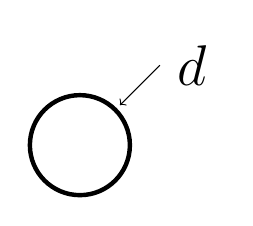
\begin{tikzpicture}[x=0.5in, y=0.5in]
\huge
	\draw[black, ultra thick] (0,0) circle (0.5);
	%\draw[black, ultra thick] (0,0) circle (0.35);
	\draw[->] (0.8,0.8) -- (0.4,0.4) node[pos=0,right]{$d$};
	%\draw[->] (0.6,-0.6) -- (0.4,-0.4) node[pos=0,right]{$t$};
	%\draw[->] (0.1,-0.1) -- (0.2,-0.2);
\end{tikzpicture}
\caption{Round tube}
\end{subfigure}
\begin{subfigure}[b]{.35\linewidth}
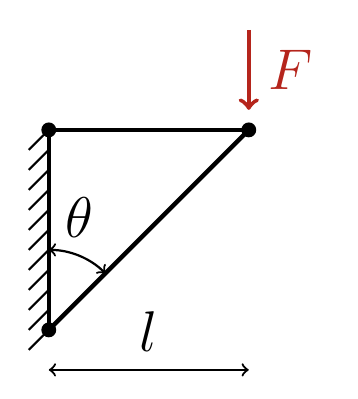
\begin{tikzpicture}[x=1in, y=1in]
\huge
	\draw[black, ultra thick] (0,0)--(1,0)  node[circle,fill,pos=1,scale = 0.3]{};
	\draw[black, ultra thick] (1,0)--(0,-1) node[circle,fill,pos=1,scale = 0.3]{};
	\draw[black, ultra thick] (0,-1)--(0,0) node[circle,fill,pos=1,scale = 0.3]{};
	
	\draw[->, BrickRed, ultra thick] (1,0.5)--(1,0.1) node[pos=0.5, right]{$F$};
	
	\draw[<->, black, thick] (0,-1.2)--(1,-1.2) node[pos=0.5, above]{$l$};
	\draw[<->, black, thick] (0,-0.6) arc (90:45:0.4) node[pos=0.5, above]{$\theta$};
	\draw[black, thick] (0,0)--(-0.1,-0.1);
	\draw[black, thick] (0,-0.1)--(-0.1,-0.2);
	\draw[black, thick] (0,-0.2)--(-0.1,-0.3);
	\draw[black, thick] (0,-0.3)--(-0.1,-0.4);
	\draw[black, thick] (0,-0.4)--(-0.1,-0.5);
	\draw[black, thick] (0,-0.5)--(-0.1,-0.6);
	\draw[black, thick] (0,-0.6)--(-0.1,-0.7);
	\draw[black, thick] (0,-0.7)--(-0.1,-0.8);
	\draw[black, thick] (0,-0.8)--(-0.1,-0.9);
	\draw[black, thick] (0,-0.9)--(-0.1,-1.0);
	\draw[black, thick] (0,-1.0)--(-0.1,-1.1);
	
\end{tikzpicture}
\caption{Trussed structure}
\end{subfigure}
\begin{subfigure}[b]{.35\linewidth}
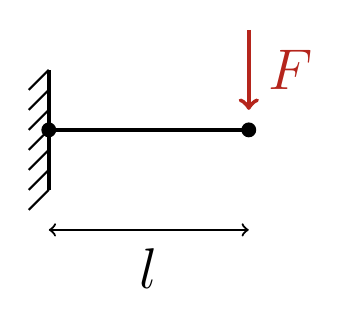
\begin{tikzpicture}[x=1in, y=1in]
\huge
	\draw[black, ultra thick] (0,0)--(1,0)  node[circle,fill,pos=1,scale = 0.3]{};
	\draw[black, ultra thick] (0,-.3)--(0,0) node[circle,fill,pos=1,scale = 0.3]{};
	\draw[black, ultra thick] (0,0)--(0,0.3);
	
	\draw[->, BrickRed, ultra thick] (1,0.5)--(1,0.1) node[pos=0.5, right]{$F$};
	
	\draw[<->, black, thick] (0,-.5)--(1,-.5) node[pos=0.5, below]{$l$};
	\draw[black, thick] (0,0.1) --(-0.1,0);
	\draw[black, thick] (0,0.2) --(-0.1,0.1);
	\draw[black, thick] (0,0.3) --(-0.1,0.2);
	\draw[black, thick] (0,0)   --(-0.1,-0.1);
	\draw[black, thick] (0,-0.1)--(-0.1,-0.2);
	\draw[black, thick] (0,-0.2)--(-0.1,-0.3);
	\draw[black, thick] (0,-0.3)--(-0.1,-0.4);
\end{tikzpicture}
\caption{Cantilevered structure}
\end{subfigure}
\caption{Trussed versus cantilevered structures.}
\end{figure}

The stress that the cantilevered beam sees varies along the cross-section as shown below.

\begin{figure}[H]
\begin{subfigure}[b]{.4\linewidth}
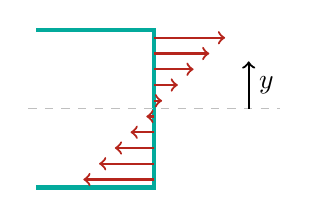
\begin{tikzpicture}
	\draw[ultra thick, JungleGreen] (-1.5,1)--(0,1)--(0,-1)--(-1.5,-1);
	\foreach \x in {0.9,0.7,...,-0.9}{
		\draw[->, thick, BrickRed] (0,\x) -- (\x, \x);
		}
	\draw[dashed, lightgray] (-1.6,0)--(1.6,0);
	\draw[->, thick] (1.2,0)--(1.2,0.6) node[pos=0.5, right]{$y$};
\end{tikzpicture}
\end{subfigure}\begin{subfigure}[b]{.5\linewidth}
\large
\begin{align}
	\sigma = \frac{M y}{I} = \frac{M}{S}
\end{align}
\end{subfigure}
\caption{Stress (red arrows) in a cantilevered beam (teal).}
\end{figure}

The stress is the highest at the outer portions of the tube, and can be found by the bending moment $M$ induced on the tube, the radius of the tube $y$ and moment of inertia $I$, or the section modulus $S$. You can conduct your own research into these if you want, but an important takeaway from this is that increasing the diameter of the tube will have a huge impact on $I$, so we'd ideally want a very large $I$.

For our example of a round bar,
\begin{align}
%	I = \frac{\pi}{64}(d^4 - (d-t)^4)
%	S = \frac{\pi}{32 d}(d^4 - (d-t)^4)
	I = \frac{\pi}{64}d^4 \\
	S = \frac{\pi}{32}d^3
\end{align}

and in our cantilevered structure, the bending moment at the base is simply $M = F \ l$. This means that we can find the maximum stress as:

\begin{align}
	\sigma_{cantilever} = \frac{F l}{\frac{\pi}{32}d^3}
\end{align}

Which isn't very meaningful until we compare that to the trussed structure.

For the trussed structure, we will assume that all the joints are pinned, so the members of it act as links. This isn't a particularly realistic assumption, but it is in some ways a conservative one. We can then analyze the node where the force $F$ is applied.

\begin{figure}[H]
\begin{subfigure}[b]{.4\linewidth}
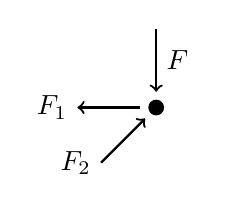
\begin{tikzpicture}
	\fill[black] (0,0) circle (0.1);
	\draw[->, thick] (0, 1) -- (0, 0.2) node [pos=0.5, right]{$F$};
	\draw[->, thick] (-0.2, 0) -- (-1, 0) node[pos=1, left]{$F_1$};
	\draw[->, thick] (-0.7,-0.7) -- (-0.14,-0.14) node[pos=0,left]{$F_2$};
\end{tikzpicture}
\end{subfigure}\begin{subfigure}[b]{.5\linewidth}
\begin{align}
	\sum F_x &= 0 \ \ \rightarrow & F_2 cos(\theta) - F &= 0 \\
	\sum F_y &= 0 \ \ \rightarrow & F_1 - F_2 sin(\theta) &= 0
\end{align}
\end{subfigure}
\caption{Free-body diagram for node of force application.}
\end{figure}

We can then solve for the forces in the links:

\begin{align}
	F_1 &= F tan(\theta) \\
	F_2 &= F \frac{1}{cos(\theta)}
\end{align}

For simple links like these, the stress is simply the force in the link, divided by the cross-sectional area.

\begin{align}
	\sigma_{truss, 1} &= \frac{F}{\frac{\pi}{4} d^2} \ tan (\theta) = \frac{F}{\frac{\pi}{4} d^2} \frac{sin(\theta)}{cos(\theta)} \\
	\sigma_{truss, 2} &= \frac{F}{\frac{\pi}{4} d^2} \frac{1}{cos(\theta)} & 
\end{align}

This isn't immediately comparable to the cantilever, as it doesn't have $l$ in its expression, and the cantilever example doesn't have $\theta$. But we can consider the example of:

\begin{table}[]
\begin{tabular}{llll}
$F$       & $d$      & $\theta$      & $l$     \\
$100$ lbf & $0.5$ in & $30$ degrees & $10$ in
\end{tabular}
\end{table}

\begin{align}
	\sigma_{truss, 1} &= \frac{100 \ \mbox{lbf}}{\frac{\pi}{4} (0.5 \ \mbox{in})^2 } tan(30 \ \mbox{degrees}) &= 295 \ psi\\
	\sigma_{truss, 2} &= \frac{100 \ \mbox{lbf}}{\frac{\pi}{4} (0.5 \ \mbox{in})^2 } \frac{1}{cos(30 \ \mbox{degrees})} &= 588 \ psi \\
	\sigma_{cantilever} &= \frac{100 \ \mbox{lbf} \ 10 \mbox{in}}{\frac{\pi}{32} (0.5 \ \mbox{in})^3} &= 81500 \ psi
\end{align}

Those values are so extremely disparate! OK, we're using really thin rods though. If we used that additional weight we save by not having the truss support to beef up the cantilever rod though, we'd get better though, right? After all, that $d$ term is cubed in the cantilever equation!

\begin{align}
	\sigma_{cantilever} &= \frac{100 \ \mbox{lbf} \ 10 \ \mbox{in}}{\frac{\pi}{32} (1.0 \ \mbox{in})^3} &= 10185 \ psi
\end{align}

Sure, doubling the cantilever rod's diameter gets us an 8-fold decrease in stress, but we're still off by orders of magnitude from the axial case.

Indeed, designing good load paths trumps adding material every time.

\section{Big Sections}
\begin{theorem} \label{theorem:big_sections}
Wide but thin is stronger and stiffer.
\end{theorem}

Recalling the equation for bending stress,

\begin{equation*}
	\sigma = \frac{M y}{I} = \frac{M}{S}
\end{equation*}

and looking at \href{https://en.wikipedia.org/wiki/List_of_second_moments_of_area}{\color{red}\underline{a number of shapes and their equation for $I$}},

 we notice that the moment of inertia $I$ grows roughly with the cube of the tube diameter. If we think about this and the geometry, that would mean that in a piece of tubing with the same cross-sectional area, we could get a greater $I$ by maximizing the diameter and minimizing the wall thickness. There is a problem with taking this to an extreme (consider the humble aluminum beverage can), but in general, the effect of increasing the diameter of a section dwarfs the effect of increasing the thickness by the same relative amount.

The same is also true of shafts in torsion / carrying torque.

Additionally, notice how multiple moments of inertia are listed for some shapes. Consider a piece of rectangular box tube. It can be bent in two orientations. One has a much larger effective diameter, so is the stronger and stiffer direction. Consider the orientation you lay tube when making structures.

\section{Minimize, Centralize, and Lower Mass}

\begin{theorem} \label{theorem:lower_mass}
	The most sstable and agile vehicle is a small point mass on the floor.
\end{theorem}

\begin{figure}
	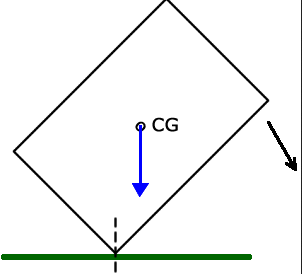
\includegraphics[width=0.5\textwidth]{imgs/cg_explanation.png}
	\caption{Center of gravity of an object about to tip}
\end{figure}

Minimizing the center of gravity of mobile platforms is almost always an extremely important design consideration, as it is what determines the fundamental tipping characteristics of the platform. For a non-accelerating and free-standing object, if the center of gravity passes outside of the support base of the object, it will begin to fall. For accelerating objectss, a higher center of gravity will tend to make the object tilt against the direction of acceleration, increasing the likelihood of tipping.

Minimizing overall mass is often a desirable goal, as decreased mass will make the same amount of force result in quicker acceleration, or require less force for the same acceleration. This will either reduce the time spent doing something, or the energy required to do it.

Centralizing mass can also be desirable, although the effect is often less pronounced. An object with spread-out mass is much harder to accelerate rotationally versus one with concentrated mass (even of the same mass), again, meaning higher centralization will facilitate lower energy consumption or decreased time-to-target.

\section{Spread the Base}

\begin{theorem} \label{theorem:spread_base}
The wider the base, the more stable.
\end{theorem}

Similar to how increasing the diameter of a section increases strength, so does increasing the diameter of bolt patterns, sprockets, gears, and just about anything that transfers load.

Increasing the diameter has another benefit beyond strength, and that is backlash.

%TODO: simple calculation showing how loads are resolved (see the minesota FLL for a simple example)

\begin{figure}
	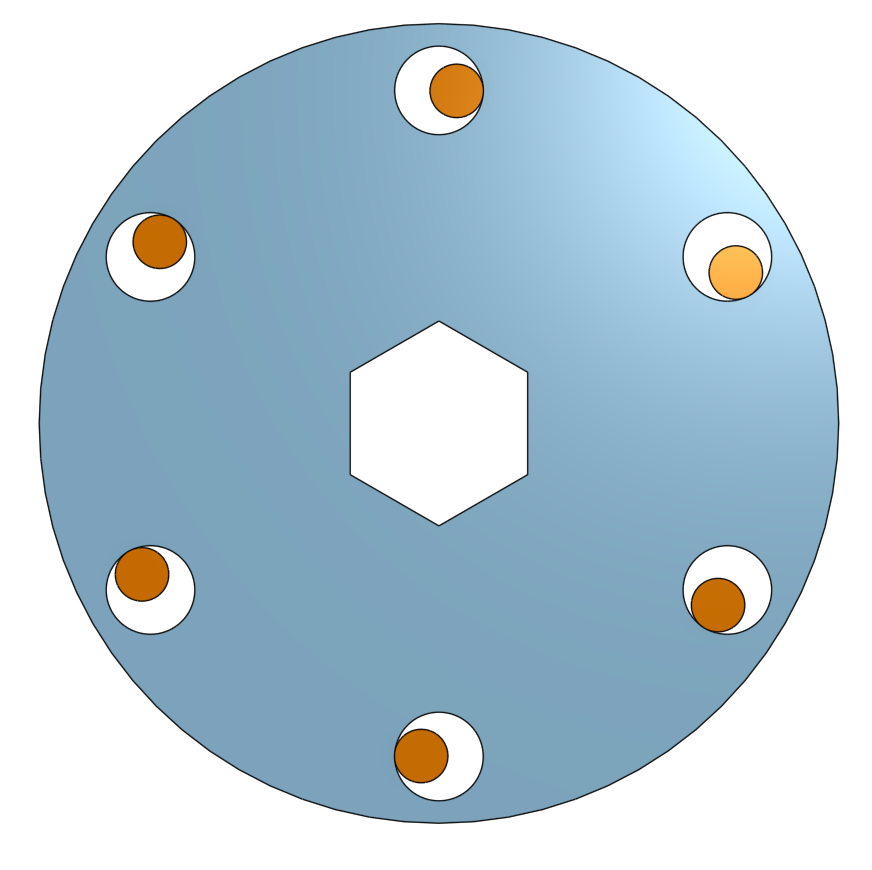
\includegraphics[width=0.5\textwidth]{imgs/hub_tolerance.png}
	\caption{Loose-fitting pins (orange) in a hub (blue).}
\end{figure}

Consider the pins in a hub illustrated above. While a bit exaggerated, clearance between components is necessary to ease assembly, and to deal with manufacturing tolerances. These clearances and tolerances are generally fixed with respect to the diameter of the bolt circle, however. We could minimize the angular slop in this assembly by increasing the diameter.

An interesting conclusion of theorems \ref{theorem:load_paths} and \ref{theorem:spread_base} is that using a linear actuator of some sort on a pivoting mechanism can be more precise and strong than one driven by a rotary actuator at its pivot point.

\section{Abbe Error}

\textit{Abbe error}\index{Abbe/sine error}, or \textit{sine error} refers to the error that can come about when parts are not aligned angularly as they were expected to be.

\begin{figure}[H]
	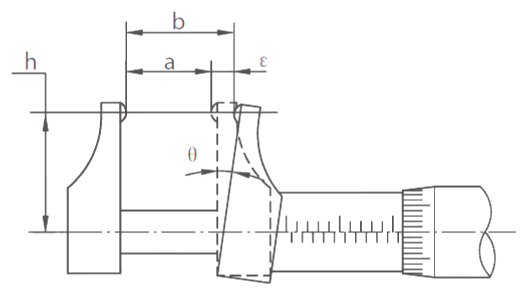
\includegraphics[width=0.6\textwidth]{imgs/abbe_error.png}
	\caption{Abbe error on a micrometer.}
\end{figure}

The error is equal to:

\begin{align}
	error = h \ sin(\theta) \approx h \ \theta \ \mbox{(for small $\theta$)}
\end{align}

Expressed verbally this means that

\begin{theorem} \label{theorem:abbe}
Angularity adds up, proportional to the distance.
\end{theorem}

If precision matters, minimize the angular error of your mechanism, or minimize the lever arm associated with the angular error.


\section{Tolerance Stacking}

Consider stacking multiple blocks that are all $10 \pm 1$ mm thick to achieve a height of $100$ mm. We would need 10 blocks, and so the error would compound among each block, up to $\pm 10$ mm! Clearly, one singular component would be better, even if it had a lower tolerance of even $\pm 5$ mm.

Considering also that more components means more cost, and more potential weak links,

\begin{theorem}
Minimize the number of components.
\end{theorem}

\section{Loosening}

\textit{Positive retention}\index{positive retention} is ensuring that vibrations and loads will not effect the positioning of components. This means avoiding slots for adjustment (that do not have additional locking schemes like cams), and bolts that must be ``just properly tightened" in order to work properly.

We discussed a number of mechanisms for keeping bolts from loosening under vibration in section \ref{subsec:threads}. Most of these solutions don't cost much to implement. There's generally no reason not to do them. And so,

\begin{theorem}
Positive retention is awesome, let's do more of that.
\end{theorem}

\section{Poka-Yoke}

\begin{figure}[H]
	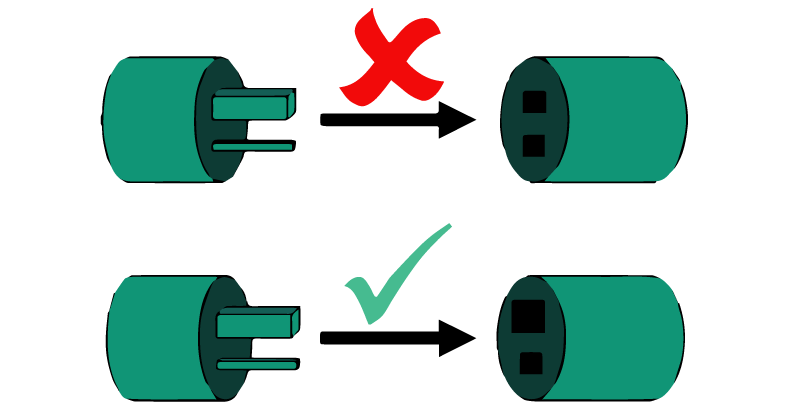
\includegraphics[width=0.7\textwidth]{imgs/poka_yoke.png}
\end{figure}

\textit{Poka-yoke}\index{poka-yoke} is Japanese for ``idiot-proofing". It refers to designing processes that cannot be messed up, or at least not without warning. Think of plugs that cannot be installed backwards, or a shaft that has a special keying on it to ensure proper clocking. Even the brightest of us can be idiots in the moment, so in short,

\begin{theorem}
If someone can screw it up, don't let them.
\end{theorem}	

\textit{Commonizing} the types and sizes of fasteners is also useful for field service and production-line efficiency. Reducing the number of part and tool sizes which a technician must carry can greatly improve productivity, as does reducing the number of different parts which must be purchased, stocked, and inventoried. This is why oftentimes on mass-produced products some fasteners seem grossly oversized- if you look closely, you may see other nearby fasteners which use the same size head, or even the exact same bolt. Even in competitive environments, the technician effort saved by using a larger but common bolt size can make the difference between making the next match and not- making up for the weight increase in spades.


\section{Design for Manufacture, Assembly, Service, and Tuning}

\begin{theorem}
	Don't make techs hate you.
\end{theorem}

The parts for your machine need to be built. After they're built, they need to be assembled together. After assembly, they will be serviced at some point. One of your objectives as an engineer is to not make the people involved with this process frustrated. If you can add a little bit of material, or avoid making a strange hole, for the sake of your machinist, do it. The many things you can do to make manufacture easy depend on the processes being used.

Designing for assembly and service is a little more straightforward. There are a few general principles:
\begin{asparaitem}
	\item Provide clearance for tools (wrenches, sockets, and rivet guns) both in the axial and radial directions.
	\item Commonize the tools needed to put a system together. If you need to use both 1/4" and \#10 screws, use button head 1/4" and socket head \#10, so that the same allen wrench can be used. Better yet, just use all 1/4" or \#10.
	\item Maximize the number of ways the assembly can be put together. At least do this at the higher levels. You shouldn't need to remove 30 pounds of machine to tighten a screw. Another way to think about this is ``design for random assembly order".
	\item Prioritize the common service routines. If a certain bolt is going to be loosened/removed a lot, make sure it's easy to get to.
\end{asparaitem}

Designing for tuning can save you hours of valuable test time. If you foresee that a mechanism will need to be adjusted, try to ensure that adjustments are simple to make, and that the adjustment can be measured and recorded in a lab manual for reference.
\begin{asparaitem}
	\item Quick pins are the ultimate in quick adjustment. The new position is immediately evident, adjustment doesn't require a tool, and there is no concern of loosening.
	\item Slotted shims, depending on how they are placed, can be a good option for adjustment. They allow the tuner to write down at a glance what the current position and newly adjusted position are for testing. However, a set of shims is required to make adjustments- meaning that the machine is not self-contained and requires a special toolkit. They also cannot be used to adjust under preload (i.e. adjusting suspension on a car while it is on the ground).
	\item Tie rods are a simple option for adjustment in many cases. Unlike shims or pins, though, they do not provide any inherent feedback about where they have been adjusted to. The eye-to-eye length could be measured and recorded, but this requires additional tools and may be prone to error.
	\item Slotted holes (by themselves) are poor methods of adjustment (See: ``Loosening"). They can be improved by using a set screw to push against the part in the slot and provide positive positioning. Like tie rods, they do not provide any inherent information about where they have been adjusted to.
	\item Set screws to clamp on rods are awful methods of adjustment. They are extremely prone to loosening... but can be useful for prototypes. They come with (or can be made to have) different tips that are more suited to frequent or infrequent adjustment.
\end{asparaitem}

\chapter{Choosing Motors and Gear Ratios}

 {\slshape \scshape ``Power is worthless, if improperly wielded."}
 
These last chapters will walk through some analysis required to actually design systems.

For any system powered by motors we may have a number of concerns.
 \index{cycle}
 \index{sprint}
\begin{asparaenum}[a)]
	\item How fast we can get from one point to another: \textit{cycle} or \textit{sprint} time.
	\item How much electrical energy or current is consumed during the maneuver.
	\item Maximizing how much force can be pushed in a worst-case scenario.
	\item Achieving a target velocity in a given time.
	\item Achieving all of these goals, for various different targets (e.g. different cycle distances).
\end{asparaenum}

This chapter covers how we can use some calculations to design a system with the right amount of motors and an appropriate gear ratio to achieve your targets.

\section{What Do Gears Really Do?}

If we have a motor with a pinion of $N_m$ teeth, mating with a driven gear of $N_d$ teeth, we would achieve a gear ratio of

\begin{align}
  G = \frac{N_d}{N_m} = \frac{\omega_m}{\omega_d} = \frac{T_d}{T_m}
\end{align}

This also works with belts or sprockets and chain (though you may need to keep an eye on the direction of rotation, as gears can reverse the direction of rotation).


\begin{figure}[H] \centering
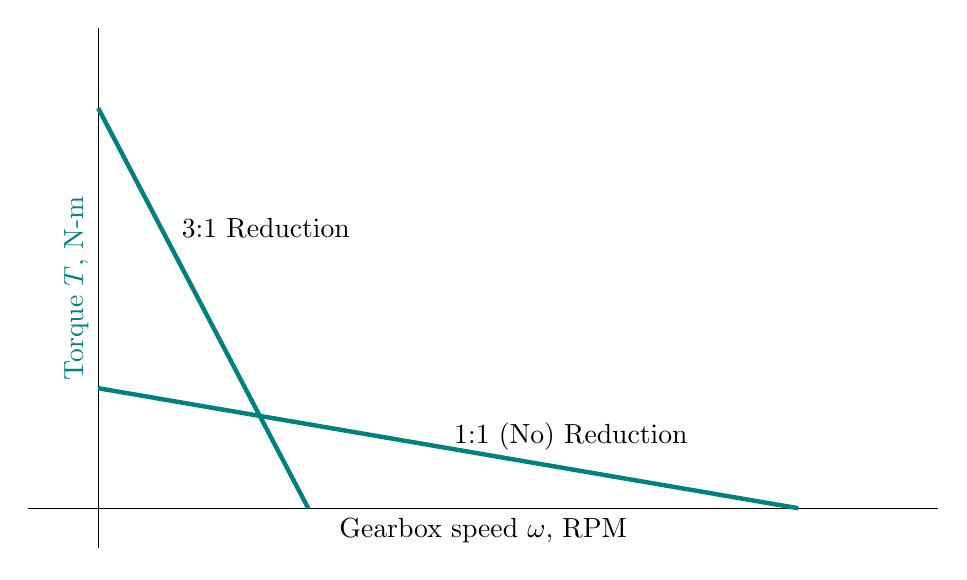
\begin{tikzpicture}[x=3.5in,y=2.0in]
  %\fill[lightgray] (1.0,0)--(0,1.0)--(0,0)--cycle;
  \draw[black] (-0.1,0)--(1.2,0) node[pos=0.5,below]{Gearbox speed $\omega$, RPM};
  \draw[black] (0,-0.1)--(0,1.2) node[pos=0.5,above,rotate=90,teal]{Torque $T$, N-m};

  \draw[teal, ultra thick] (1.0,0)--(0,0.3) node[pos=0.6, right, black]{\ \ \ \ \ \ \ 1:1 (No) Reduction};
  \draw[teal, ultra thick] (0.3,0)--(0,1.0) node[pos=0.7, right, black]{\ 3:1 Reduction};
\end{tikzpicture}
\caption{A 3:1 gear reduction shifts the effective motor curve of a gearbox.}
\end{figure}

The 3:1 ratio reduces maximum speed, but increases the maximum torque. It also changes the RPM at which maximum power and efficiency occur. A gearbox that has too much gear-down:
\begin{asparaitem}
	\item Quickly gets up to its maximum speed and remains there throughout the majority of its action.
	\item Operates beyond the speed necessary for peak efficiency of the motor.
	\item Operates for too long, wasting electrical power.
\end{asparaitem}

Whereas a gearbox that is not geared down enough:
\begin{asparaitem}
	\item Operates below the speed necessary for peak power or efficiency of the motor.
	\item Pulls excessive current, wasting electrical power.
	\item May not even move at all in the first place, lacking the strength to overcome load placed on it.
\end{asparaitem}

But how do we know that we've geared appropriately? We could definitely test all the different ratios, gather all the operating data, and then draw a conclusion... or we could do some preemptive math. Don't worry- you don't even need to get your hands too dirty. All of the rough stuff has been done already- you just need to know how to use the design applications to get the answer you want.

But knowing roughly what's going on is important. There's an old joke in engineering,

 {\slshape \scshape ``All data is wrong. But this data, having gone through an incredibly sophisticated computer, is somehow ennobled and none dare question it."}
 
 Which roughly translates to: ``You can't just mash buttons and trust the results".

\section{Developing a Generalized Mechanism Model}

\subsection{The Simple Flywheel Case}

Let's examine a simple case of a motor accelerating a flywheel. This is also (essentially) the same as any system with no friction or gravity-fighting (like an ideal drivetrain).
	
	\begin{figure}[H] \centering
	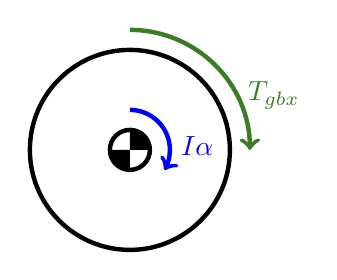
\begin{tikzpicture}[x=1.0in,y=1.0in]
		\draw[ultra thick] (0,0) circle (0.1);
		\fill[black] (0,0.1)--(0,0)--(0.1,0) arc[start angle=0, end angle=90, radius=0.1]--cycle;
		\fill[black] (0,-0.1)--(0,0)--(-0.1,0) arc[start angle=180, end angle=270, radius=0.1]--cycle;
		\draw[ultra thick, black] (0,0) circle (0.5);
		
		%\draw[ultra thick, red, ->] (0,0.6) arc[start angle=90, end angle=180, radius=0.6] node[pos=0.7,left]{$M_{resist}$};
		\draw[ultra thick, OliveGreen, ->] (0,0.6) arc[start angle=90, end angle=0, radius=0.6] node[pos=0.7,right]{$T_{gbx}$};
		
		\draw[ultra thick, blue, ->] (0,0.2) arc[start angle=90, end angle=-30, radius=0.2] node[pos=0.7,right]{$I \alpha$};
	\end{tikzpicture}	
	\caption{Free-body diagram of the flywheel}
	\end{figure}	
	
	We can apply conservation of angular momentum to the flywheel.
	\begin{align}
		%\sum M &= I \alpha + \cancelto{0 \ \mbox{(no mass transfer)}}{\sum \dot{m}(...)} \\
		T_{gbx} &= I \ \alpha_{wheel}
	\end{align}
	
	This tells us about the rate of acceleration $\alpha$, but what about the velocity $\omega$? 
		
	\begin{align}
		\alpha_{wheel} &= \frac{d \omega_{wheel}}{dt} \\
		\omega_{motor} &= G \omega_{wheel} \\
		G T_{stall} \frac{\omega_{free} - \omega}{\omega_{free}} &= \frac{I}{G} \frac{d \omega}{dt}
	\end{align}
	
		This is a ``differential equation" ($\frac{d \omega}{dt}$ and $\omega$ appear in the same equation). These are tricky to solve. \textit{There be dragons ahead. If you don't care to know all the intricate mathy details, skim ahead. I don't blame you.}
		
	\subsection{The Full-Blown Calculus Approach}
	
	We can solve differential equations with calculus!	
	\begin{align}
		\mbox{let }& &B  &= \frac{G^2 T_{stall}}{I} \\
		\mbox{Substitute: }& & B\ \frac{\omega_{free} - \omega}{\omega_{free}} &= \frac{d \omega}{d t} \\
		\mbox{Separate and integrate: }& & \int B\ dt &= \int \frac{\omega_{free}}{\omega_{free} - \omega} d \omega \\
		\mbox{Compute integral (introduces $C$): }& & B t + C &= -\omega_{free}\ ln[\omega_{free} - \omega] \\
		\mbox{Solve for $\omega$: }& & \omega &= \omega_{free} - C\ e^{-\frac{B t}{\omega{max}}} \\
		\mbox{Solve for C with initial condition }& & \omega(0) &= 0 \rightarrow C = \omega_{free} \\
		& &\omega &= \omega_{free}\ [1 - e^{-\frac{G^2\ T_{stall}\ t}{I\ \omega{max}}}] \\
		& &\omega_{gbx} &= \frac{\omega_{free}}{G}\ [1 - e^{-\frac{G^2\ T_{stall}\ t}{I\ \omega{max}}}]
	\end{align}	
	
	If we plot this algebraic solution with some generalized values, we can start to investigate what it really means.	
	
	\begin{figure}[H] \centering
	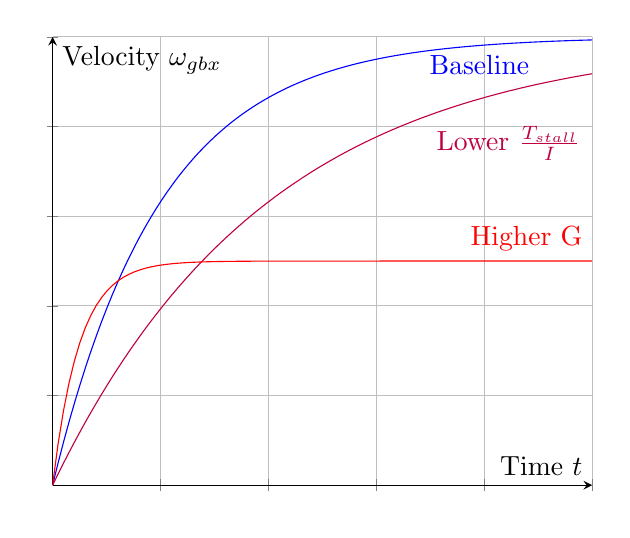
\begin{tikzpicture}[x=3.0in,y=1.5in]
		%\draw[gray] (0,0)--(3,0) node[pos=0.5,below,black]{Time $t$};
		%\draw[gray] (0,0)--(0,2) node[pos=0.5,above,rotate=90,black]{Ang. Velocity $\omega_{gbx}$};
		
		%\draw[red] (0,0)
		
		\begin{axis}[grid=both,
          xmax=5,ymax=1,
          xticklabel=\empty, yticklabel=\empty,
          axis lines=middle,
          restrict y to domain=-7:12,
          xlabel={Time $t$},
          ylabel={Velocity $\omega_{gbx}$}
          ]
		\addplot[blue,domain=0:5,samples=100]  {1*(1-exp(-1^2*x))} node[pos=0.8,below] {Baseline};
		\addplot[purple,domain=0:5,samples=100]  {1*(1-exp(-1^2/2*x))} node[pos=0.7,below right] {Lower $\frac{T_{stall}}{I}$};
		\addplot[red,domain=0:5,samples=100]  {1/2*(1-exp(-2^2*x))} node[above left] {Higher G};
		\end{axis}
	\end{tikzpicture}
	\caption{Flywheel example solution, with different representative parameters}
	\end{figure}
		
	This assumes that there is no constant load, or friction.
	This behavior is generally true, but not exactly true.
	
	\subsection{A Brute-Force Approach}
	We don't need to solve that differential equation using calculus. Or math. We can use basic arithmetic and computers to simulate it! We can do this with a 'numeric differential equation solver', like Euler's Method:
	\begin{equation}
		\frac{d}{dt} f(t) \approx \frac{\Delta f(t)}{\Delta t}
	\end{equation}\begin{equation}
		f(t_{i+1}) = f(t_{i}) + \frac{d}{dt}[f(t_{i})]\ {\Delta t}
	\end{equation}
	
	\begin{figure}[H]
		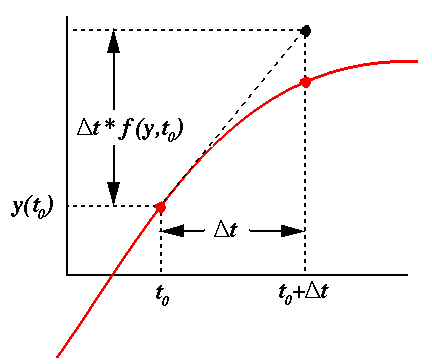
\includegraphics[width=0.35\textwidth]{imgs/euler_method.png}
		\caption{Graphical representation of Euler's method.}
	\end{figure}
	
	Another way of putting it... ``the next value is the current value, plus the rate of change times the timestep of the simulation". 	We just need to get an expression for the $\frac{d}{dt}f(t)$ we are interested in, and write some code that will repeat this process with a small enough $\Delta t$. This process is sometimes called 'discretization' since we are taking a continuous field of time $t$ and separating it into little $\Delta t$ chunks.	
		
	Let's go back to our flywheel example, and add resistance $M_{resist}$ to it. This $M_{resist}$ can be anything- it can represent friction, air resistance, a spring, you name it! The numeric simulation approach makes this trivial.
	
	\begin{figure}[H] \centering
	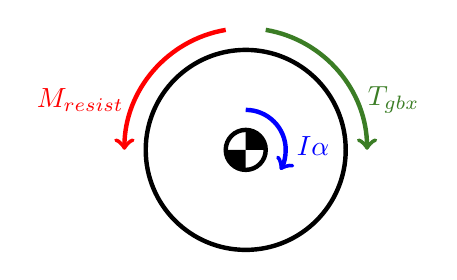
\begin{tikzpicture}[x=1.0in,y=1.0in]
		\draw[ultra thick] (0,0) circle (0.1);
		\fill[black] (0,0.1)--(0,0)--(0.1,0) arc[start angle=0, end angle=90, radius=0.1]--cycle;
		\fill[black] (0,-0.1)--(0,0)--(-0.1,0) arc[start angle=180, end angle=270, radius=0.1]--cycle;
		\draw[ultra thick, black] (0,0) circle (0.5);
		
		\draw[ultra thick, red, ->] (-0.1,0.6) arc[start angle=99.6, end angle=180, radius=0.608] node[pos=0.7,left]{$M_{resist}$};
		\draw[ultra thick, OliveGreen, ->] (0.1,0.6) arc[start angle=80.4, end angle=0, radius=0.608] node[pos=0.7,right]{$T_{gbx}$};
		
		\draw[ultra thick, blue, ->] (0,0.2) arc[start angle=90, end angle=-30, radius=0.2] node[pos=0.7,right]{$I \alpha$};
	\end{tikzpicture}	
	\caption{Free-body diagram for the flywheel, with additional resistance $M_{resist}$.}
	\end{figure}
	
	We can go through and repeat the same analysis as before.
	\begin{align}
		%\sum M &= I \alpha + \cancelto{0 \ \mbox{(no mass transfer)}}{\sum \dot{m}(...)}  \\
		T_{gbx} - M_{resist} &= I \alpha_{wheel} \\
		\alpha_{wheel} &= \frac{d}{dt} \omega_{wheel} \\
	\end{align}
	
We can solve to yield the equations we need to perform Euler's method:	
	
	\begin{align}
		\frac{d}{dt} \omega_{wheel} &= \frac{T_{gbx} - M_{resist}}{I} \\
		\frac{d}{dt} \theta_{wheel} &= \omega_{wheel}
	\end{align}
	
	My \href{http://thaddeus-maximus.github.io/swissarmyengineer/}{\color{red}\underline{EveryCalc}}\index{EveryCalc!simple mechanism} tool contains a Simple Mechanism Calculator you can use to leverage these physics.

	
\section{Using the Simulations: Analysis/Optimization Examples}

Let's consider an example drivetrain, with 4 NEOs, 8" diameter wheels, weighing about 143 pounds, meeting 30 N of resistive force. We want to go 10 meters. We have two gear ratio options to consider: a 10:1 gearbox, and a 7:1 gearbox. Which should we pick?

Before you look at the plots, go to the simulator and plug in those values, see if you can come up with an answer of which gets to the destination faster.

\clearpage
	
	\begin{figure}[H] \centering
	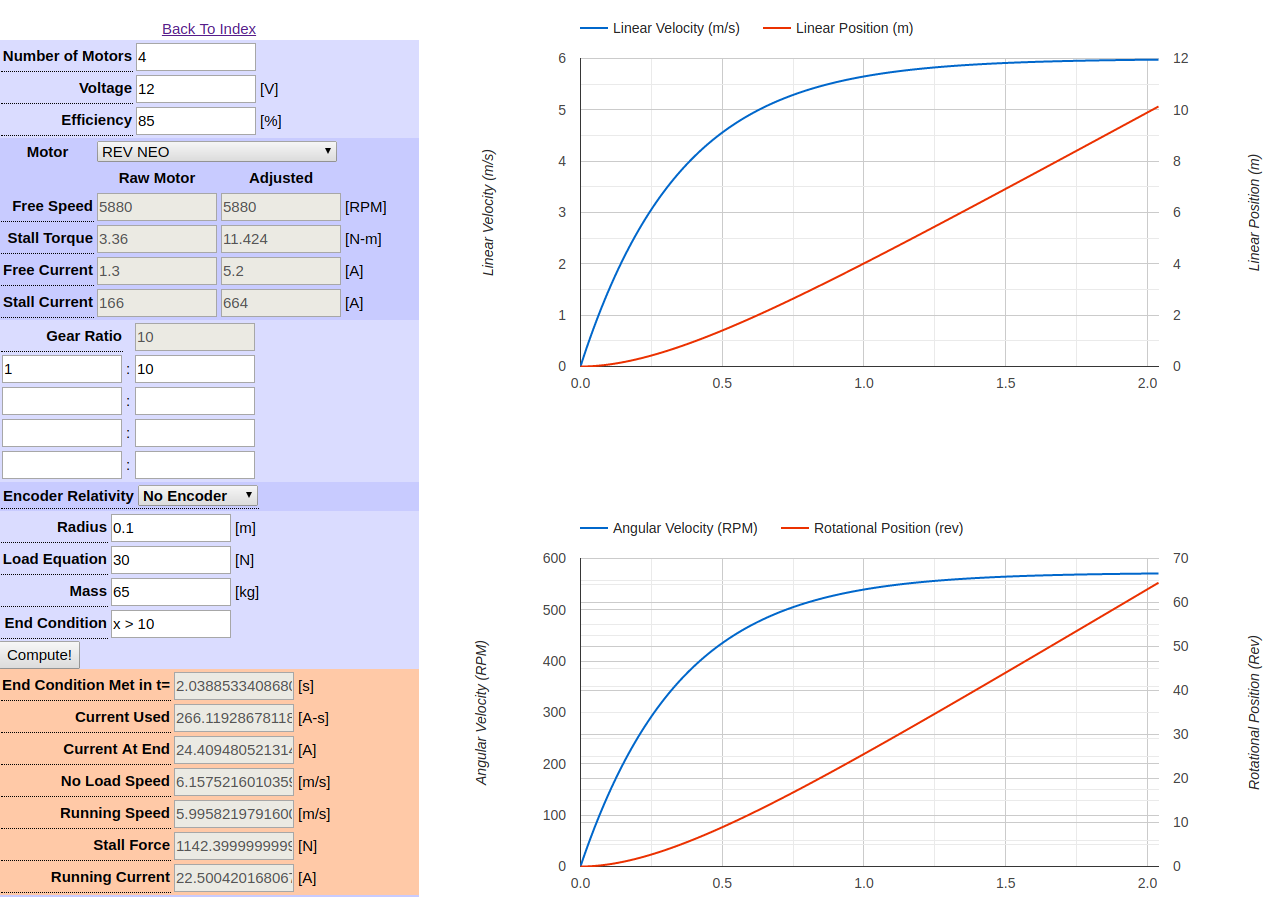
\includegraphics[width=0.8\textwidth]{imgs/thsae_1.png}
	\caption{Baseline simulation, G = 10, t = 2.03 s}
	\end{figure}
	
	\begin{figure}[H] \centering
	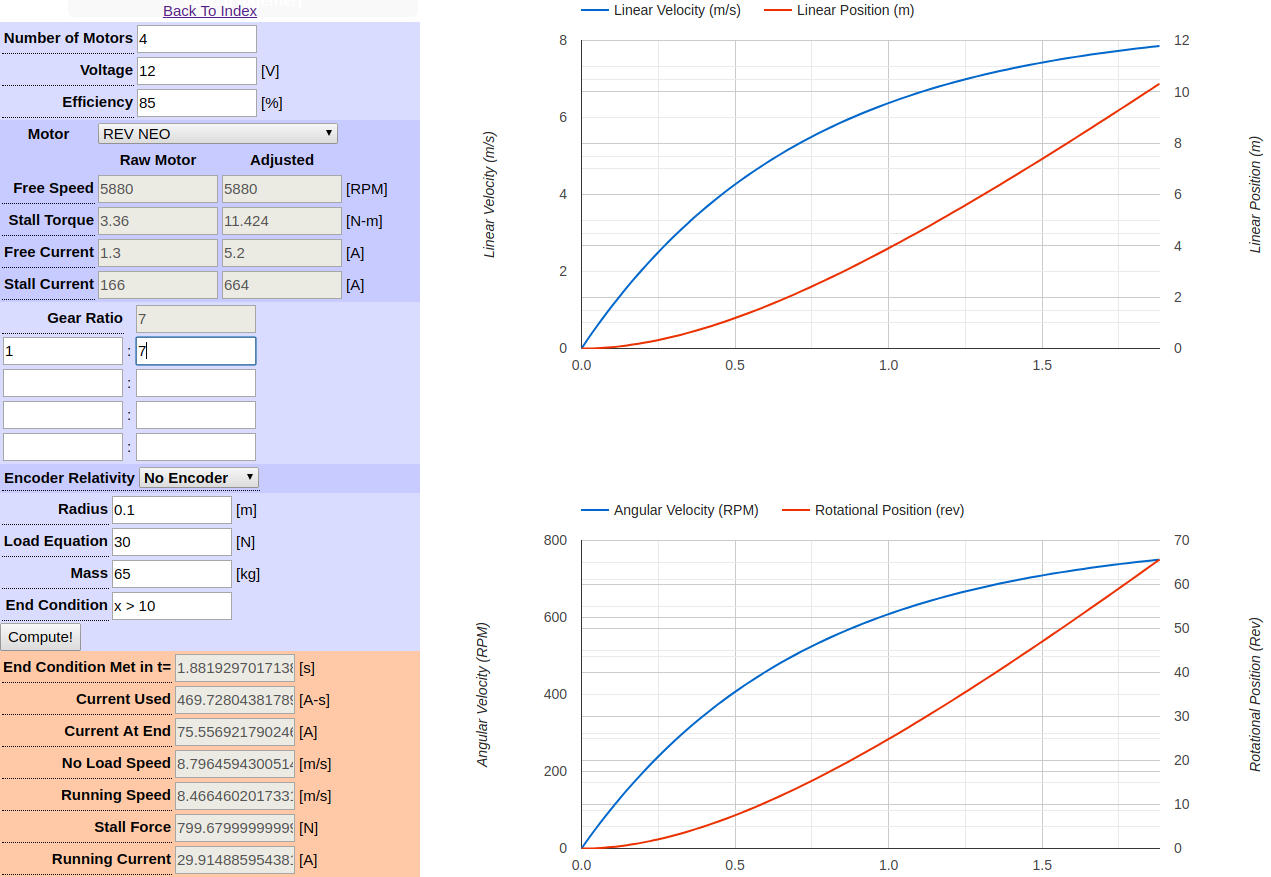
\includegraphics[width=0.8\textwidth]{imgs/thsae_2.png}
	\caption{Alternative simulation, G = 7, t = 1.88 s}
	\end{figure}
	
	It looks like the ratio of 7 will get to our destination faster!
	
	However, maybe this isn't our only concern. Drivetrains are complex mechanisms with many objectives (as we'll discuss later). This simulator uses a similar approach as discussed above to compute energy consumption, and it turns out that the G = 10 case has lower current consumption (almost half!) in this maneuver. It has more initial pushing power. It also gets to positions less than 3 meters away faster. There are a lot of trade-offs!
	
	The calculator won't give you the right answer right off the bat, but it does free you from thinking about the numbers and math too much so you can focus on making system-level decisions, which is something that a computer can't quite so easily do.
	
